\begin{XeClass}{FsPermission}
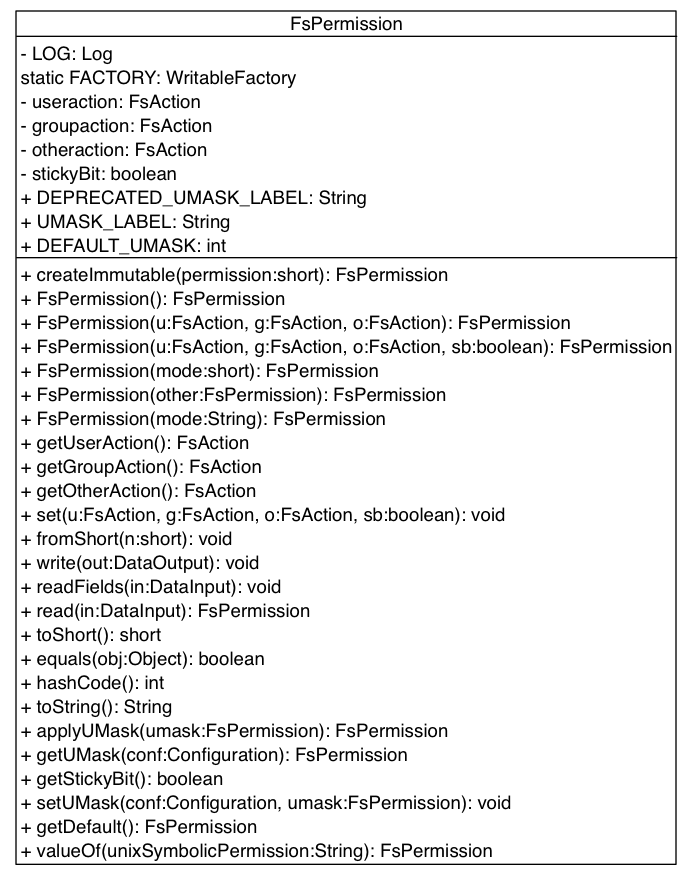
\includegraphics[width=10cm]{cdig/FsPermission.png}
     
 虽然前缀是Fs, 但与文件系统并没有太多关联.
 组合3个对象以表示完整的权限模式.
 3个对象分别是用户行为、所属组行为和其他行为所对应的权限

    \begin{XeMethod}{\XePublic}{FsPermission}{createImmutable}
         
 Create an immutable \emph{FsPermission} object.
 创建一个不可变的FsPermission对象

    \end{XeMethod}

    \begin{XeMethod}{\XePublic}{FsAction}{getUserAction}
         
 Return user \emph{FsAction}.
 获取用户行为权限

    \end{XeMethod}

    \begin{XeMethod}{\XePublic}{FsAction}{getGroupAction}
         
 Return group \emph{FsAction}.
 获取所属组行为权限

    \end{XeMethod}

    \begin{XeMethod}{\XePublic}{FsAction}{getOtherAction}
         
 Return other \emph{FsAction}.
 获取其他行为权限

    \end{XeMethod}

    \begin{XeMethod}{\XePrivate}{void}{set}
         
 设置3个行为权限

    \end{XeMethod}

    \begin{XeMethod}{\XePublic}{void}{fromShort}
         
 从short模式设置权限

    \end{XeMethod}

    \begin{XeMethod}{\XePublic}{short}{toShort}
         
 Encode the object to a short.
 解码权限到short模式

    \end{XeMethod}

    \begin{XeMethod}{\XePublic}{boolean}{equals}
         
 {@inheritDoc}判断行为权限是否相等

    \end{XeMethod}

    \begin{XeMethod}{\XePublic}{FsPermission}{applyUMask}
         
 Apply a umask to this permission and return a new one
 应用umask到权限的设置,并返回一个新的权限

    \end{XeMethod}

    \begin{XeMethod}{\XePublic}{FsPermission}{getUMask}
         
 Get the user file creation mask (umask)
 获取用户文件的umask{@code UMASK_LABEL} config param has umask value that is either symbolic
 or octal.
 Symbolic umask is applied relative to file mode creation mask;
 the permission op characters '+' clears the corresponding bit in the mask,
 '-' sets bits in the mask.
 Octal umask, the specified bits are set in the file mode creation mask.{@code DEPRECATED_UMASK_LABEL} config param has umask value set to decimal.

    \end{XeMethod}

    \begin{XeMethod}{\XePublic}{void}{setUMask}
         
 Set the user file creation mask (umask)
 设置用户文件的umask

    \end{XeMethod}

    \begin{XeMethod}{\XePublic}{FsPermission}{getDefault}
         
 Get the default permission.
 获取默认权限,short模式下为00777

    \end{XeMethod}

    \begin{XeMethod}{\XePublic}{FsPermission}{valueOf}
         
 Create a FsPermission from a Unix symbolic permission string
 从Unix符号权限字符串创建一个文件系统权限对象

    \end{XeMethod}

\end{XeClass}
